\chapter{Eye Model}
\label{chap:eyeModel}

A very important step in hardware and software development is testing. For an eye tracking system it requires a big effort to do this with real data as the information where the participant looks at each time needs to be recorded alongside of the videostream. For this project real time data processing is needed as there is no hardware available on GazelleCompute to encode or store four streams of 120fps with QVGA resolutioni

To optimize the algorithms a simple way of generating new data where the gaze direction and the camera positions are known, would simplify the process. 
\section{What is Important}
\label{sec:whatIsImportant}

The 3D-Modeling software to create the model needs to fulfill a few requirements:
\begin{itemize}
	\item Correct representation of refracting light
	\item Create animations 
	\item Be scriptable
	\begin{itemize}
		\item Set position and rotation of certain objects at a certain frame
		\item Set camera properties and which camera is active
		\item Read the position and rotation of objects at any frame
	\end{itemize}
	\item (optional)Be free
	\item (optional)Run on Linux
	\begin{itemize}
		\item Server that can be used to render runs Linux containers
	\end{itemize}
	\item (optional)Be easy to learn
\end{itemize}

Blender is able to match all requirements although the last one might be debatable. You can apply a material properties to a surface. This includes refracting. Rotation and position of objects can be inserted as keyframes and it interpolates the steps in-between. 

Blender is also an open source project that is built with Python and has an powerful API that gives access to nearly everything.

\section{The Human Eye}
A side view of a human eye model is visible in \ref{fig:humanEyeModel}. The camera can only see the front part of the eye. As a result only the cornea, anterior chamber and the iris need to be modeled correctly. The lens can be simplified by a black surface. 

It might be counterintuitive that the cornea extends as much out of the eyeball as visible in \ref{fig:humanEyeModel}. An easy way to verify is to close the eye and move the eyes while holding a finger on the eyelid.
\label{sec:theHumanEye}
\begin{figure}[H]
	\centering
	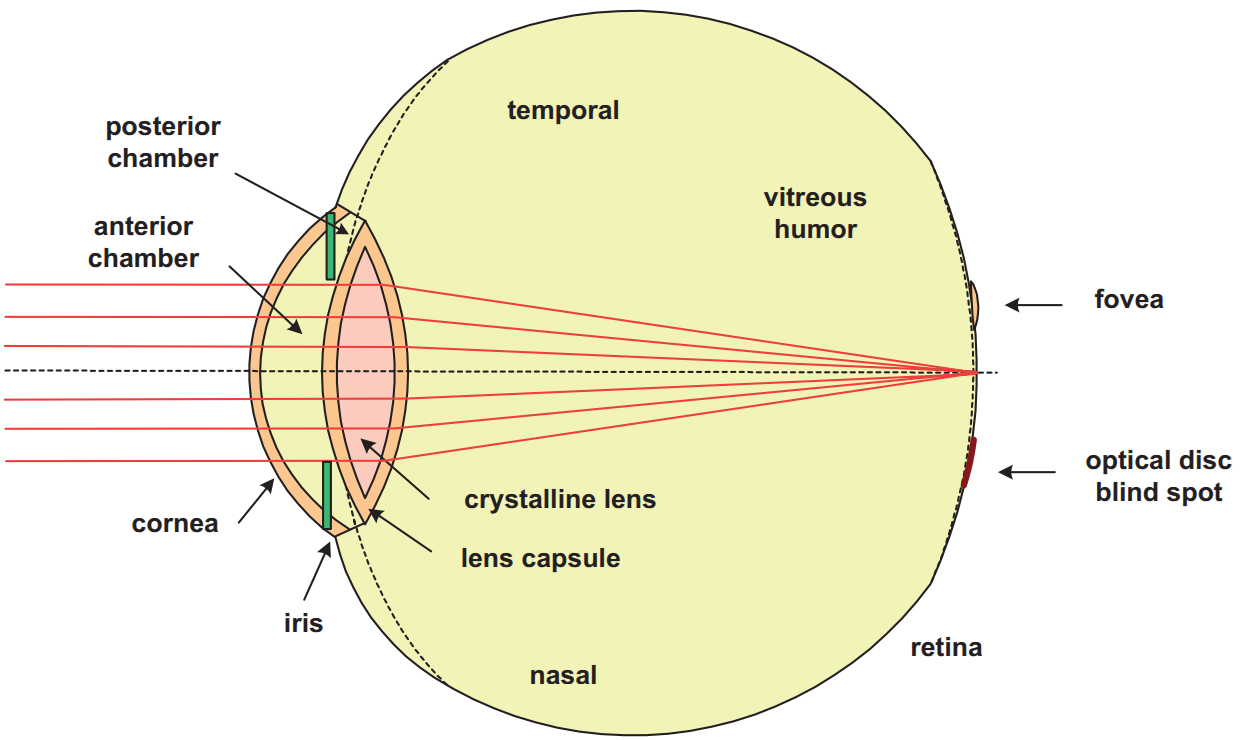
\includegraphics[scale=0.3]{images/human_eye_model.png}
	\caption{Side view of a human eye model}
	\label{fig:humanEyeModel}
\end{figure}

There are a few models with different values for the refracting indexes, radii and distances but they are close together in most cases. So the simplified Gullstrand eye was chosen.
\begin{table}[!htb]
\centering
\begin{tabular}{@{}|l|l|l|l|l|l|l|@{}}
	\hline
	
	\multirow{2}{*}{} & \multicolumn{3}{l|}{\thead{Relaxed}} & \multicolumn{3}{l|}{\thead{Accomodated}} \\ \hhline{~------}
	\thead{ Notaton\\{}} &  \thead{Radius r \\ {}[mm] }        & \thead{Thickness d\\ {}[mm]}    & \thead{Index n\\ {}}        & \thead{Radius r \\ {}[mm] }& \thead{Thickness d \\ {}[mm] }& \thead{Index n\\{} }    \\ \hline
	cornea     &  7.70        & 0.50      & 1.376       &  7.70   &0.50  & 1.376\\ \hline
	anterior chamber & 6.80        & 3.10     & 1.336       & 6.80    & 2.70&1.336 \\ \hline
	crystalline lens     &  10.0    & 3.60          & 1.4085    & 5.33   &   4.0  &  1.426 \\ \hline
	vitreous humor    p  & -6.00      & 17.187         & 1.336    & -5.33  & 13.816  &  1.336  \\ \hline
\end{tabular}
\caption{Algorithmic Complexity of the associative Qt Containers where each element can be accessed over the associated key}
\label{tab:qt-container-associative}
\end{table}


\subsection{Demonstrandum}
\label{subsec:satzspiegeltest_typoblindtext_demonstrandum}

Quod erat demonstrandum. Seit 1975 fehlen in den meisten Testtexten die Zahlen, weswegen nach TypoGb. 204 \S ab dem Jahr 2034 Zahlen in 86 der Texte zur Pflicht werden. Nichteinhaltung wird mit bis zu 245 \texteuro oder 368\$ bestraft. Genauso wichtig in sind mittlerweile auch \^A\c{c}c\`e\~nt\"e, die in neueren Schriften aber fast immer enthalten sind. Ein wichtiges aber schwierig zu integrierendes Feld sind OpenType-Funktionalit\"aten. Je nach Software und Voreinstellungen k\"onnen eingebaute Kapit\"alchen, Kerning oder Ligaturen (sehr pfiffig) nicht richtig dargestellt werden.

\subsubsection{Subsubsection}

This is a typo dummy text. On it you can see if all the letters there are and how they look. Sometimes one uses words like Hamburgefonts, Rafgenduks or Handgloves to test fonts. Sometimes phrases that contain all letters of the alphabet - one calls these sets "pangrams". 

\subsubsection{Subsubsection}

Well known is this: The quick brown fox jumps over the lazy old dog. Often in type dummy texts also foreign-language sentence parts are installed (AVAIL\textsuperscript{\texttrademark} and Wefox\textsuperscript{\textregistered} are testing aussi la Kerning) to test the effect in other languages. In Latin, for example, almost every font looks good. Quod erat demonstrandum.

\section{Webstandards}
\label{sec:satzspiegeltest_webstandards}

Everywhere the same old story. The layout is complete, the text is slow in coming. This layout is now not naked in space and small and empty occurs, I help out: the dummy text. Created exactly for this purpose, always in the shadow of my big brother "Lorem Ipsum", I look forward every time you read a few lines. Because esse est percipi - being is to be perceived.

And now because you already have the goodness to accompany me a few more sentences long, I would like to take this opportunity to serve you not only as a stopgap, but to point out something that is going to be perceived as deserved: Web viz. See Web standards are the rules that build on the websites. So there are rules for HTML, CSS, JavaScript or XML, words that you might have heard of your developers. These standards ensure that all parties the maximum benefit from a website.

\begin{figure}[H]
	\centering
		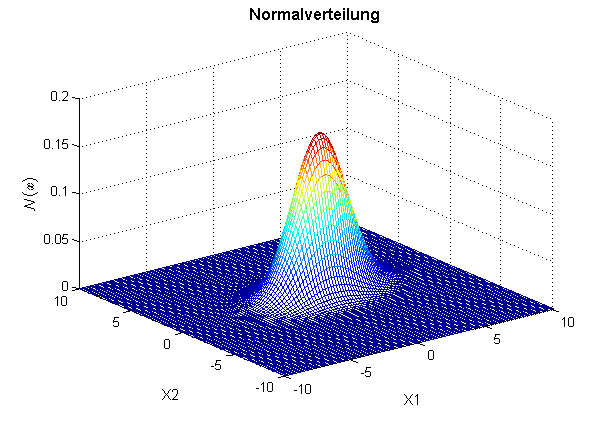
\includegraphics[scale=0.7]{images/multivariate_gauss.png}
	\caption{Normal distribution}
	\label{fig:normal_distribution}
\end{figure}

In contrast to previous websites we no longer need, for example, two different sites for the program Internet Explorer and another browser. It extends a page that - properly applied - both works on different browsers on the net, but just as good for printing or display on a cell phone is. Mind: A site for all formats. What a relief. Standards save time provide for the development costs and ensure that web pages can be easier to maintain later. Of course, only if everyone adheres to these standards.
